\begin{figure*}[!ht]
    \centering
    \begin{minipage}[l]{0.29\linewidth}
        \centering
        \hspace{-1cm}
        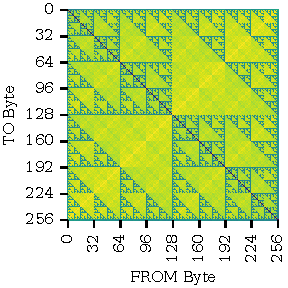
\includegraphics[width=\linewidth]{fig/images/pdf/single-byte-sierpinski-perfect-hw.pdf}
        \subcaption{}
    \end{minipage}\hfill
    \begin{minipage}[c]{0.69\linewidth}
        \centering
        \hspace{0.5cm}
        
\includegraphics[width=\linewidth]{fig/images/pdf/single-byte-sierpinski-heatmaps.pdf}
        \subcaption{}
    \end{minipage}
    \Description{Heatmaps of all 1-byte transition latencies under various initial word-level states. The x-axis is the \textit{FROM byte}, or the initial state of the transitioning byte and the y-axis is the TO-byte, or the state the transitioning byte transitions into. A Sierpinski gasket appears as a fractal of isosceles triangles where all triangle bases face away from the diagonal line extending from the upper left to the lower right of each heat-mapped square. A reference Sierpinski gasket is shown on the left, and two rows of measured patterns are shown on the right, where each row contains heat-maps for 1 product for every column represents the latencies for a specific initial word and target byte configuration. These experimental measurements show Sierpinski-like patterns where traces of triangles appeared to be punctured. The triangle traces are the darker colors corresponding to a lower write latency, whereas the lighter colors are faster write latencies. Puncturing therefore corresponds to an expected low write latency becoming higher. This puncturing is less noticeable for the 4Mb chips and nearly erases the pattern completely for the 8Mb chips.}
    \caption{A reference Sierpinski gasket with an added Hamming weight bias (left) and the corresponding minimum 1-byte transition write latencies $t_{ws}$ averaged across all chips (right) for $G=\mathbf{0}$ and $G=\mathbf{0}$ at two byte indices.}
    \label{fig:1B-sierpinski-scan}
\end{figure*}
